\section{Porous Media}
\subsection{Author and source}
The porous media test-case is derived from the paper \cite{Aarnes_2007}. A copy of the source code is included in the \texttt{git} repository, with some minor modifications to run the 3D version of the model, as described below. The application is a finite volume code that simulates a toy model of a reservoir.
\subsection{Description of the mathematical formulation}\label{power_cont_adj_math}
Detailed mathematical formulation is given in \cite{Aarnes_2007}
\subsection{Directory structure and description of files}
The porous media test-case is organized into following directories and subdirectories:\\

\dirtree{%
.1 /. 
.2 MATLAB\DTcomment{Original files with some modifications for 3D}.
.3 MATLAB/data\DTcomment{Data about the reservoir}.
.3 MATLAB/2phase\DTcomment{Saturation solver and drivers for 2-phase simulator}.
.3 MATLAB/TPFA\DTcomment{Two-point flux approximation method}. 
.3 MATLAB/MFEM\DTcomment{Mixed finite element method}. 
.2 Fortran\DTcomment{Fortran version of porous media model}. 
.3 Fortran/Port\DTcomment{Port of the \texttt{MATLAB} version}. 
.3 Fortran/DiscreteAdj/OpenAD/joint\DTcomment{Incomplete OAD version}. 
}
\hfill\break
\noindent Some of the descriptions for the \texttt{MATLAB} directories were obtained from the \texttt{README} file that comes with the original code.
\subsubsection{\texttt{MATLAB} version}
%The directory \texttt{MATLAB} contains the original files with some minor bug fixes to comply with \cite{Rao_2013} and \cite{Sandu_2012}. The \texttt{MATLAB} version of the code uses the continuous adjoint formulation as mentioned in the earlier references.\\
%
%\noindent The listing of files and their descriptions follow.\\
%\dirtree{%
%.1 /. 
%.2 MATLAB.  
%.3 main.m\DTcomment{Driver file for the power generation model}. 
%.3 sens\_check.m\DTcomment{Model with continuous adjoint}. 
%.3 TSOPF\_Experiments.pdf\DTcomment{Same as \cite{Rao_2013}}. 
%}
%\hfill\break
%\noindent The \texttt{MATLAB} version can be executed like below.\\
%
%\begin{lstlisting}[language=mymatlab, numbers=none]
%>> main
%\end{lstlisting}
%\hfill \break
%\noindent The plots generated by the \texttt{MATLAB} version appear on the following page.
%\clearpage
%\begin{figure}[h]
%\centering
%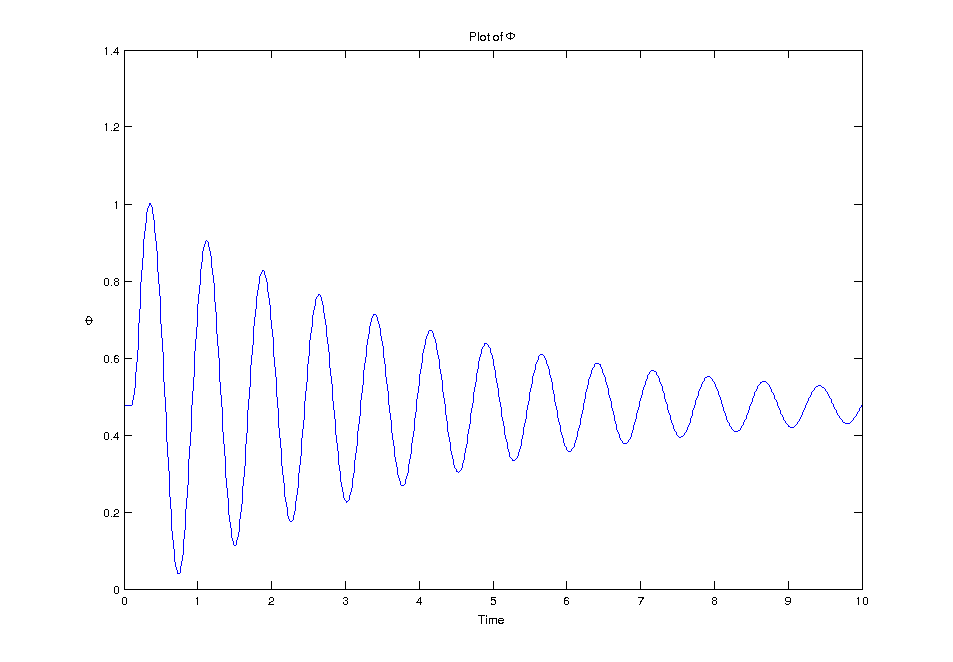
\includegraphics[width=1.2\linewidth]{../Code/miniApps/power_grid/phi_matlab.png}
%\label{fig:plot_of_phi_matlab}
%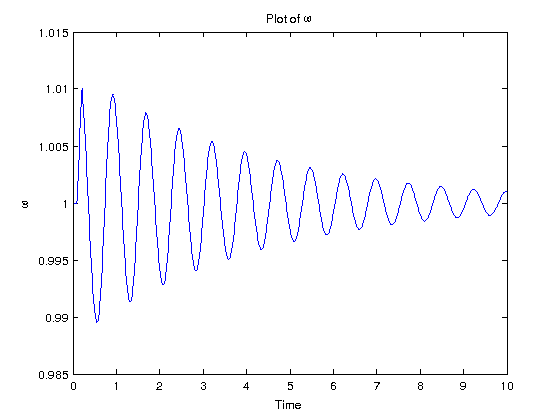
\includegraphics[width=1.2\linewidth]{../Code/miniApps/power_grid/omega_matlab.png}
%\label{fig:plot_of_omega_matlab}
%\end{figure}
\clearpage
\subsubsection{\texttt{Fortran} port}\label{sec_fortran_port_porous}
%The directory \texttt{Fortran/ContinousAdj} contains the port of the \texttt{MATLAB} version. L-BFGS \cite{Byrd_1996},\cite{Zhu_1997},\cite{Morales_2011} was used to perform the optimization in the \texttt{Fortran} port, a copy of which can be obtained \href{http://users.iems.northwestern.edu/~nocedal/lbfgsb.html}{here}.\\
%
%\noindent The directory \texttt{Fortran/ContinousAdj} contains the files to compile continous adjoint version of the optimal control problem listed in \ref{power_cont_adj_math} and \cite{Rao_2013}. The binaries (\textbf{files}), corresponding to these, on building the directory are \texttt{powergrid} (\textbf{{main.f90}}).\\
%
%\noindent The listing of files and their descriptions follow.\\
%
%\dirtree{%
%.1 /. 
%.2 Fortran/ContinuousAdj.  
%.3 blas.f\DTcomment{L-BFGS support file}. 
%.3 constants.f90\DTcomment{Constants and shared variables}. 
%.3 gnufor2.f90\DTcomment{\texttt{Fortran} bindings for GNUPlot}. 
%.3 iterate.dat\DTcomment{Output from L-BFGS optimization routine}. 
%.3 lbfgsb.f\DTcomment{L-BFGS optimization routine}. 
%.3 linpack.f\DTcomment{L-BFGS support file}. 
%.3 main.f90\DTcomment{Driver for the continuous adjoint port}. 
%.3 Makefile\DTcomment{Build commands}. 
%.3 print\_active.f\DTcomment{Routines to pretty print matrices and vectors}. 
%.3 timer.f\DTcomment{L-BFGS support file}. 
%}
%\hfill \break
%\noindent The plots generated by the \texttt{Fortran} version using continuous adjoints appear on the following page.
%\clearpage
%\begin{figure}[h]
%\centering
%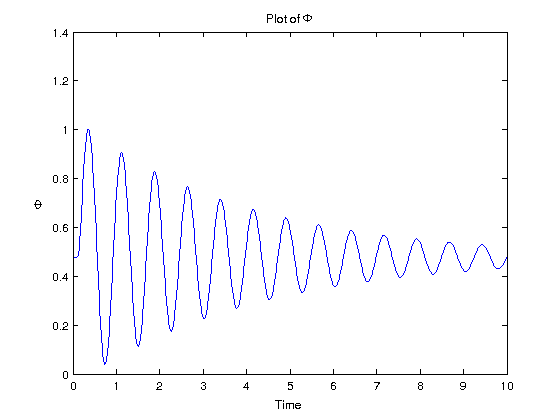
\includegraphics[width=1.2\linewidth]{../Code/miniApps/power_grid/phi_fortran_ca.png}
%\label{fig:plot_of_phi_fortran_ca}
%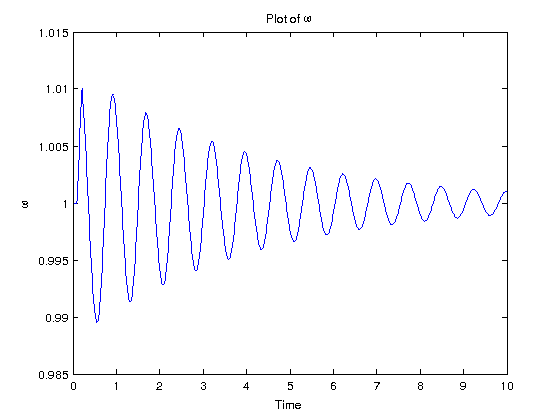
\includegraphics[width=1.2\linewidth]{../Code/miniApps/power_grid/omega_fortran_ca.png}
%\label{fig:plot_of_omega_fortran_ca}
%\end{figure}
%\clearpage
\subsubsection{\texttt{Fortran} port with \texttt{OpenAD/F} in Reverse Joint Mode}
%For details on reverse split mode refer \cite{Griewank_2008} and \cite{Utke_2014}.\\
%
%\noindent The directory \texttt{Fortran/DiscreteAdj/OpenAD/Split} contains the files to compile the discrete adjoint version of the \texttt{Fortran} port in section \ref{sec_fortran_port_power}. L-BFGS \cite{Byrd_1996},\cite{Zhu_1997},\cite{Morales_2011} was used to perform the optimization in the discrete adjoint version of the Fortran port, a copy of which can be obtained \href{http://users.iems.northwestern.edu/~nocedal/lbfgsb.html}{here}.\\
%
%\noindent The binaries (\textbf{files}), corresponding to these, on building the directory are \texttt{powergrid} (\textbf{{main.f90}}).\\
%
%\noindent The adjoint version of the forward model is used in the file  \texttt{main.f90}. These have been obtained by passing the undifferentiated routines to \texttt{OpenAD/F} in reverse-split mode.\\
%
%\noindent For details on how to call \texttt{OpenAD/F} in reverse-split mode refer \cite{Utke_2014}. The listing of files and their descriptions follow.\\
%
%\dirtree{%
%.1 /. 
%.2 Fortran/DiscreteAdj/OpenAD/Split.  
%.3 blas.f\DTcomment{L-BFGS support file}. 
%.3 constants.f90\DTcomment{Constants and shared variables}. 
%.3 gnufor2.f90\DTcomment{\texttt{Fortran} bindings for GNUPlot}. 
%.3 iterate.dat\DTcomment{Output from L-BFGS optimization routine}. 
%.3 lbfgsb.f\DTcomment{L-BFGS optimization routine}. 
%.3 linpack.f\DTcomment{L-BFGS support file}. 
%.3 main.f90\DTcomment{Driver for the discrete adjoint of port}. 
%.3 Makefile\DTcomment{Build commands}. 
%.3 Makefile\_continuous\_adjoint\DTcomment{Build commands for CA model}. 
%.3 numerics.f90\DTcomment{FW and CA model routines from \texttt{main.f90}}. 
%.3 print\_active.f\DTcomment{Routines to pretty print matrices and vectors}. 
%.3 timer.f\DTcomment{L-BFGS support file}.  
%}
%
%\hfill \break
%\noindent The plots generated by the \texttt{Fortran} version using discrete adjoints generated by \texttt{OpenAD/F} in reverse-split mode appear on the following page.
%
%\clearpage
%\begin{figure}[h]
%\centering
%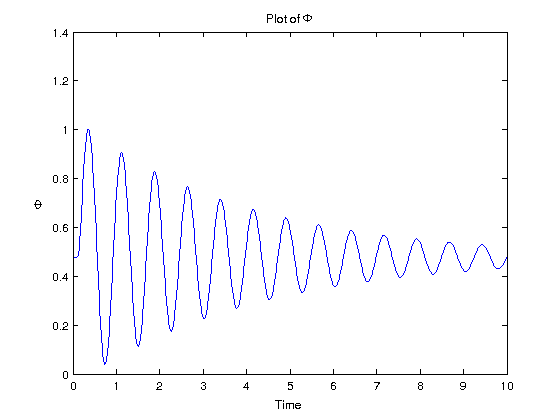
\includegraphics[width=1.2\linewidth]{../Code/miniApps/power_grid/phi_fortran_da_oad_rs.png}
%\label{fig:phi_fortran_da_oad_rs}
%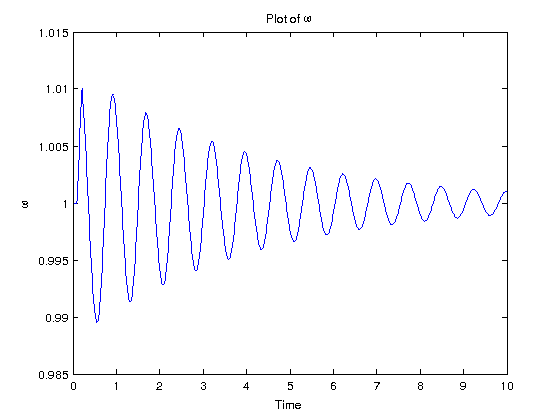
\includegraphics[width=1.2\linewidth]{../Code/miniApps/power_grid/omega_fortran_da_oad_rs.png}
%\label{fig:omega_fortran_da_oad_rs}
%\end{figure}
%\clearpage
%\subsection{Modifications performed}
\subsection{How to build}
%Running make as below, in each of the five subdirectories beginning with \texttt{Fortran/} will build the  binary \texttt{powergrid}
%\hfill\break
%\begin{lstlisting}[language=mybash, numbers=none]
%    $ make
%\end{lstlisting}
\subsection{How to verify}
%At the time of writing, there exists no script that can validate the output from any of the binaries. All versions of the binary \texttt{powergrid} should produce similar (in some sense/nearby) optimal and objective values.\\
%
%\noindent Validation by eyeballing the output from each version of the binary  \texttt{powergrid} has been performed. 
%
%\begin{TodoPar}
%\noindent It will be valuable to write a \texttt{python} script that will take as input two \texttt{csv} files and find the \texttt{max-norm} of the difference between the corresponding entries. Other norms may also be computed. 
%\end{TodoPar}
%
%\begin{HypoPar}
%\noindent I wonder it might be difficult to test the derivatives of each version of \texttt{powergrid} against another, since the code does not do computations deterministically i.e. there are convergence related iterations, each version may take different trajectories (except at the starting point) until they arrive at nearby solutions that are similar as metioned earlier.\\
%
%\noindent One solution, might be to generate multiple experiments with several different starting points and compare the derivatives at the starting points alone.
%\end{HypoPar}


%\subsection{How to extend}
